\section{Results and Discussion}

\gerald{Sepp: Can you again look into the results and check if there is any questions where academia and industry are in contradiction}
In this section, we will present the key findings from the qualitative questions of the first round of the Delphi study, the qualitative results from the second round of the Delphi study and the qualitative results from the SWOT-AHP analysis.
%\claudio{Do we only present the results of the second round (quantitative questions), or do we describe the questions we used for the first round?
%Also, should the questions be introduced in the previous section? How did we obtain those questions? Was it from the surveys? I think this information is lacking in the ``Method'' section.
%Also, we probably have to provide a rationale for each question, to show that we did not select the questions just on a hunch.
%As such, I think the method section is lacking a lot of stuff.
%We could justify the questions by saying that they are inspired by the existing survey work. This seems to be the best alternative as it is compact, and related to the surveys we introduced in the ``state of the art'' section (although we need to go back to that section and highlight more on those questions in each survey description).}

%\claudio{Are we going to disclose the list of experts?
%We need to discuss what to present here, and what to not present, to avoid overlapping with the modelica paper. 
%Alternatively, we should focus on getting the modelica paper done, and then say that this journal is the expanded version of the modelica paper. 
%I prefer this alternative.}

\claudio{Is there a way to put the information below into a picture. I think that some graphs representing the answers in each paragraph are in order. They make it a lot easier to take in the information. The text can refer to those pictures and just state facts that are inferred from the pictures (e.g., "the majority of the experts preferrer this over that..."}

\subsection{Need a name "General about co-simulation"}
Experts were asked to name which properties apply to the simulators that they have worked in co-simulation: 53 \% mentioned "The simulator approximates the solution to sets of differential equations", 22 \% "The simulator specializes in software controllers (e.g., Overture Tool)" and 22 \% "The simulator specializes in networks", 17 \% "The simulator receives input from a human-machine interface (e.g., a flight controller)", 16 \% "The simulator is a dedicated piece of hardware (e.g., a SCALEXIO)", 8 \% "The simulator specializes in finite element modelling" and  6 \% "Other".

\claudio{This paragraph seems to belong to a new section. Maybe instead of using the subsection comment to split these, we should use the paragraph command.}
To identify the main dissemination channels, experts were asked to name the three most important scientific sources to disseminate their work. 
24 \% named Modelica conference, 8 \% journal SIMULTAN, 6 \% ACM Transaction on Modeling and Computer Simulation, IEEE Transactions on Industrial Electronics, International Conference on Multibody System Dynamics, Spring Simulation Multi-conference, Workshop on Modeling and Simulation of Cyber-Physical Energy Systems and Conference on Simulation and Modeling Methodologies, Technologies and Applications.
\claudio{The above list is incomplete, right?}

\subsection{Established Standards and Tools}
To identify promising standards and tools for continuous time, discrete event and hybrid co-simulation, we asked experts (i) to give their opinion on widely accepted standards and (ii) what standard and tool they use for co-simulation. 

\begin{figure}[h!]
\centering
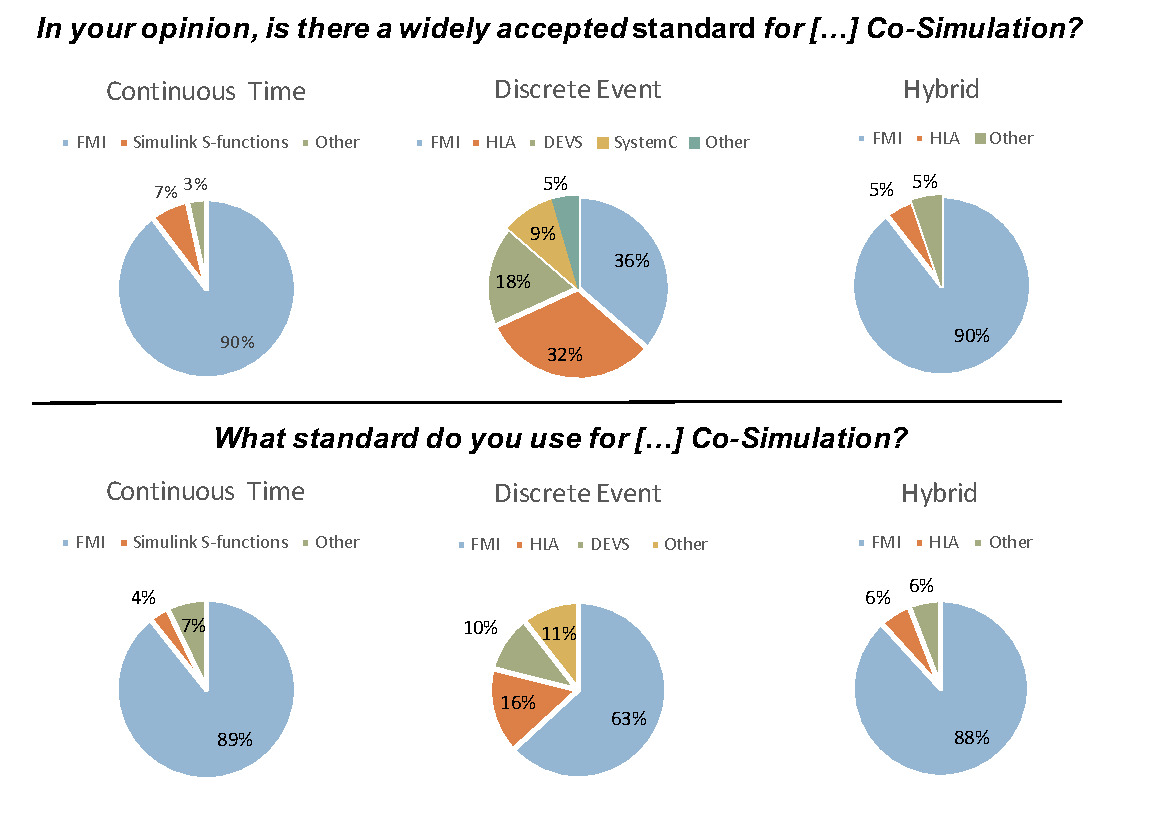
\includegraphics[width=1\textwidth]{Figures/Tools.pdf}
\caption{Widely accepted and used standards for co-Simulation. \claudio{I don't know if we mention this, but a threat to validity is the bias towards the FMI.}}
\label{fig:Standards}
\end{figure}

%\begin{figure}[h!]
%\centering
%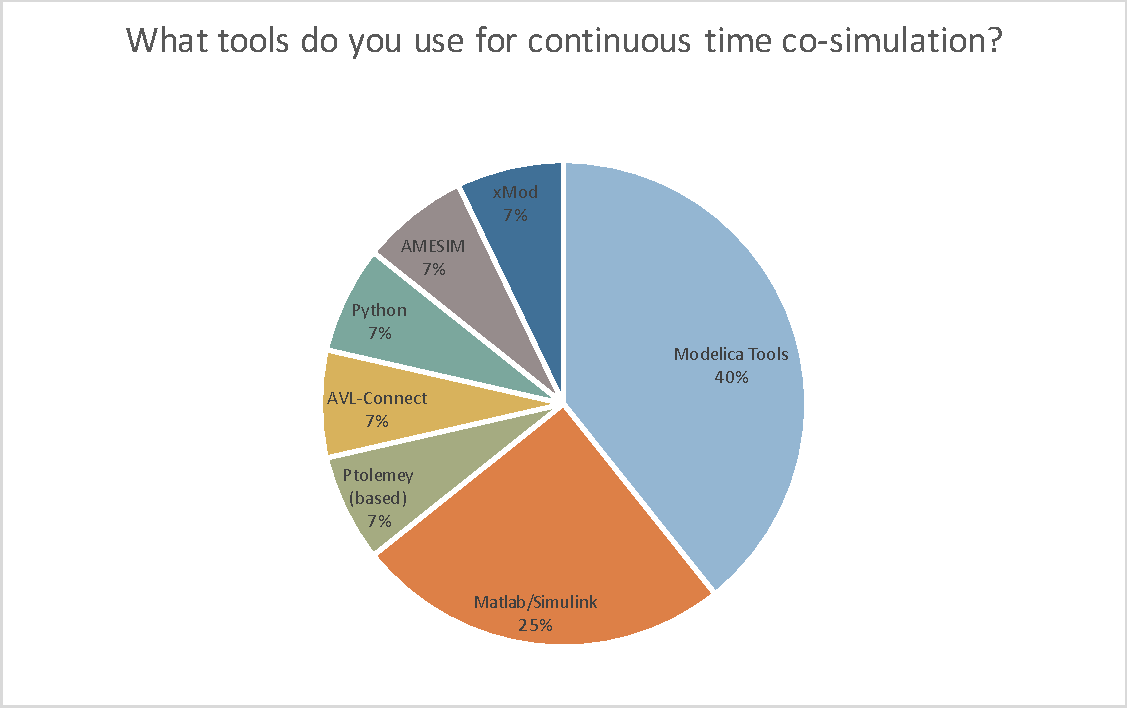
\includegraphics[width=1\textwidth]{Figures/Tools_coSim.pdf}
%\caption{Widely used tools for continuous time Co-Simulation}
%\label{fig:ToolsCont}
%\end{figure}

\claudio{We don't need the text below. It's redundant with the figure. Maybe just mention the preferred standard, and the least picked one.}
Experts in the field of co-simulation see FMI as a promising standard for continuous time, discrete event and hybrid co-simulation;  90 \% of the experts see FMI, 7 \% Simulink S-functions and 3 \% other standards as a widely accepted standard for continuous time co-simulation. 
For discrete event co-simulation  36 \% see FMI, 32 \% HLA, 18 \% DEVS formalism, 9 \% SystemC and 5 \% other standards as widely accepted. 
For hybrid so-simulation  90 \% see FMI, 5 \% HLA  and 5 \%  other standards as widely accepted. 
While for continuous time and hybrid co-simulation the responses for "widely accepted standards" and "standards which experts use" are similar, a different picture emerges for discrete event co-simulation. 
Only 36 \% of the experts state FMI as widely accepted for discrete event co-simulation; contrary to this, 63 \% of the experts use FMI for discrete event co-simulation. 
Details about research challenges and current barriers for FMI can be found in \cite{Schweiger2018b}.

In addition to promising standards, experts were asked what tools they use for co-simulation. The most common tools for continuous time co-simulation are Modelica tools and Matlab/Simulink. 
About half of the experts mentioned that they use (among other tools) \claudio{We don't need these parenthesis. It's obvious they will use other tools.} Modelica tools and about 40 \% of the experts mentioned that they use (among other tools) Matlab/Simulink. 
For discrete event co-simulation, no tool was significantly more frequently mentioned than others; very often, self-written tools were mentioned. 
Similarly, for hybrid co-simulation, no tool was significantly more frequently mentioned than others.

%\begin{figure}[h!]
%\centering
%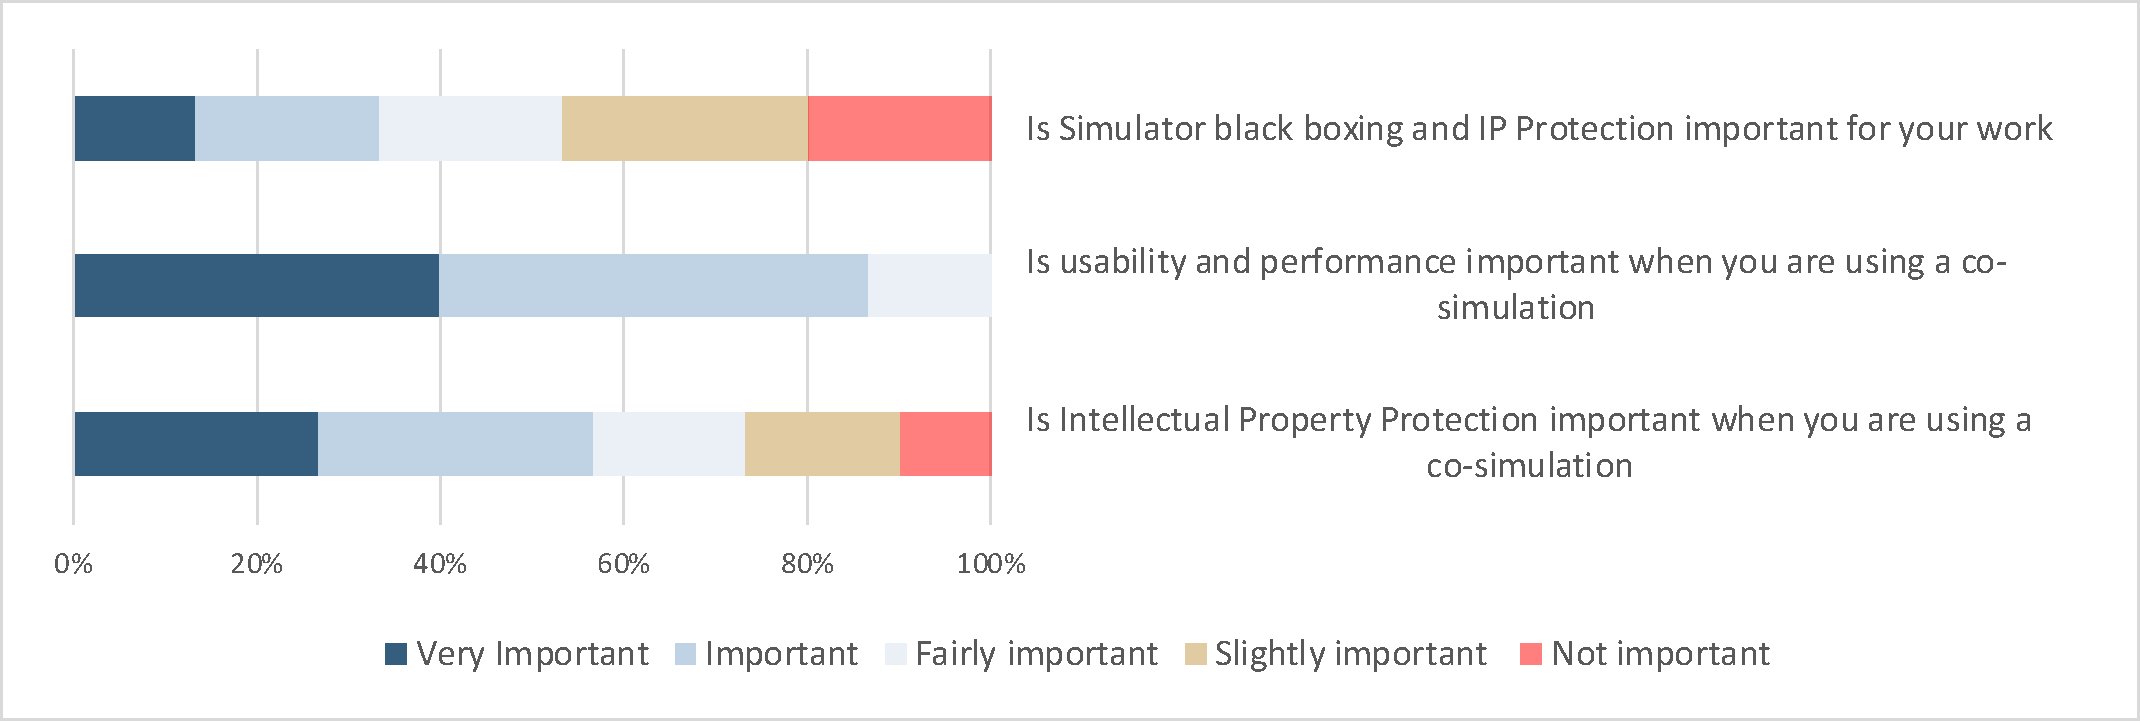
\includegraphics[width=1\textwidth]{Figures/Personal_1.pdf}
%\caption{xxxxx}
%\label{fig:xxxx}
%\end{figure}


\subsection{Current challenges}
In the first round of the Delphi study, experts commented on current challenges in co-simulation. 
Based on these responses and an extensive literature review, we formulated several statements regarding personal experiences. 
In the second round of the Delphi Study, experts were asked to rate those statements ("Have you experienced" [...]) based on a 6-point Likert scale from $1 = \text{``very frequently''}$ to $6 = \text{``never''}$. 
Table \ref{fig:challenges} summarizes the responses sorted according to how often experts experiences certain issues. 
A detailed discussion of the individual challenges goes beyond the scope of this survey; further information can be found in the references to the respective challenges in Table \ref{fig:challenges}.

\begin{table}[htbp]
\tiny
  \centering
  \caption{Experts assessments: Current challenges. Score: Very Frequently (6) Frequently (5) Occasionally (4) Rarely (3) Very Rarely (2) Never (1). \claudio{Maybe in the method section, we should explain what the interpolated median is, and how it should be interpreted. Remember that our readers are not experts in empirical studies.}}
    \begin{tabularx}{1\linewidth}{
        X
        >{\color{black}}R{0.8cm}
        >{\color{black}}R{0.8cm}
        >{\color{red}}R{0.8cm}
        <{\color{black}}
    }
    %\toprule    
    & \thead{Mean} & \thead{Median} & \thead{Interp.\\Median} \\
    \midrule
        Difficulties in practical aspects, like IT-prerequisites in cross-company collaboration  & 4.7   & 5.0   & 4.7 \\
            Difficulties due to insufficient communication between theorists and practitioners   & 4.4   & 5.0   & 4.6 \\
    Difficulties in judging the validity of a co-simulation   & 4.6   & 4.0   & 4.4 \\
    Difficulties in how to define the macro step size for a specific co-simulation \cite{Benedikt2013b,Busch2011,Gomes2017}  & 4.3   & 4.0   & 4.3 \\
        Numerical stability issues of co-simulation \cite{Busch2016,Gomes2017,Arnold2010}  & 4.4   & 4.0   & 4.3 \\
    Issues with algebraic loops \cite{Kubler2000,Gomes2017} & 4.2   & 4.0   & 4.2 \\

    Difficulties in how to define tolerances  & 4.3   & 4.0   & 4.0 \\
    Issues because of too simplistic extrapolation functions  & 3.5   & 4.0   & 3.6 \\
    Difficulties in choosing the right co-simulation orchestration algorithm (master)  & 3.6   & 3.0   & 3.4 \\
    \bottomrule
    \end{tabularx}%
   
  \label{tab:LS}%
\end{table}%

Experts frequently have \textit{"Difficulties in practical aspects, like IT-prerequisites in cross-company collaboration"} ($M=5.0; IM = 4.7$) and \textit{"Difficulties due to insufficient communication between theorists and practitioners"} ($M=5.0; IM = 4.6$). 
With the exception of \textit{"Issues because of too simplistic extrapolation functions"} and \textit{"Difficulties in choosing the right co-simulation orchestration algorithm (master)"}, all challenges are assessed by the experts with a interpolated median value greater or equal to 4 which corresponds to the answer "Occasionally"; this fact confirms that the challenges we provided are indeed challenges faced by the experts. 


\subsection{Research needs}
Based on responses in the first round of the Delphi study and an extensive literature review, experts where asked about research topics in the field of co-simulation that have not received enough attention up to now.
Table \ref{fig:ResearchNeeds} summarizes the responses which are sorted in ascending order of topics that have not received enough attention up to now. 
Based on the evaluation of the experts for each question, we have classified each topic according to whether there is a need for research: topics with an Intermediate Median score of $5.5$ or higher require ``Intensive Research Activity''.
Topics with an Interpolated Median between $5.5$ and $5.0$ require `` Moderate Research Activity'' and topics with an Interpolated Median score less than $5.0$ require `` Limited to No Research Activity''.

\gerald{link to literature (the category "Intensive Research Activity"}

\begin{table}[htbp]
\tiny
  \centering
  \caption{Experts assessments: Research needs. Score: Entirely agree (7) Mostly agree (6) Somewhat agree (5) Neither agree nor disagree (4) Somewhat disagree (3) Mostly disagree (2) Entirely disagree (1).}
    \begin{tabularx}{1\linewidth}{
        X
        >{\color{black}}R{0.8cm}
        >{\color{black}}R{0.8cm}
        >{\color{red}}R{0.8cm}
        <{\color{black}}
    }
    %\toprule    
    & \thead{Mean} & \thead{Median} & \thead{Interp.\\Median} \\
    \midrule
    Theoretical understanding of how to accurately include different kinds of controllers in different co-simulation approaches  & 5.5   & 6.0   & 5.9 \\
    Representation and enforcement of model validity assumptions  & 5.6   & 6.0   & 5.8 \\
    Hybrid co-simulation (e.g., variable structure systems, switched systems, impulsive systems, etc...)  & 5.8   & 6.0   & 5.8 \\
    Impact of coupled error controlled algorithms & 5.7   & 6.0   & 5.8 \\
    Uncertainty quantification/propagation & 5.6   & 6.0   & 5.8 \\
    Impact of updating inputs (and the discontinuity it introduces) in the subsystems  & 5.6   & 6.0   & 5.7 \\
    Acausal approaches for co-simulation  & 5.6   & 6.0   & 5.7 \\
    Impact of using different tolerances in a sub-component on the overall simulation  & 5.3   & 6.0   & 5.5 \\
    Numerical stability & 5.3   & 5.0   & 5.4 \\
    Systematic categorization of different co-simulation approaches, including a better understanding of how their model of computations and requirements overlap and differ & 5.2   & 5.0   & 5.4 \\
    Usability and performance  & 4.9   & 5.0   & 5.1 \\
    Simultaneous events  & 5.7   & 6.0   & 5.8 \\
    Integration of a wide variety of simulators despite different structures (while achieving/maintaining high performance)  & 4.8   & 5.0   & 4.9 \\
    Parallelization  & 4.6   & 5.0   & 4.9 \\
    Simulator black boxing and IP Protection & 4.1   & 4.0   & 4.1 \\


    \bottomrule
    \end{tabularx}%
   
  \label{tab:Research}%
\end{table}%

To (i) evaluate controversial assessments regarding research needs from the first Delphi round and from literature as well as to (ii) provide a different perspective on research needs, additional questions to the questions in \ref{tab:Research} were defined. 
Experts where asked if several statements are important for their work. The average score of each Likert-scale question (Very important=5 to Not important=1) was calculated. 
The statements $S_1$ \textit{"Is usability and performance important when you are using a co-simulation"} ($Mean = 4.3, M = 4.0, IM = 4.3)$) and $S_2$: \textit{"Is Intellectual Property Protection important when you are using a co-simulation"} ($Mean = 3.9, M = 4.0, IM = 3.7)$) were assessed as important.
Compared to the previous, \textit{"Is Simulator black boxing and IP Protection important for your work"} was assessed as not so important ($Mean = 3.5, M = 3.0, IM = 2.7)$).

\gerald{An expert mentioned: This connects to the fundamental idea of what is the idea (or goal) with hybrid co-simulation? Is the intention to allow, with hybrid co-simulation, the same flexibility as there is in a monolithic simulation (with everything that this entails)? To me co-simulation should be about coupling of "large" subsystems - not for instance being able to connect a circuit with resistors as separate subsystems. I image that the two different views will have very different requirements on a hybrid co-simulation. My view is also that most of this is largely unexplored and needs more research regarding the numerical properties with such a scheme."}

\gerald{"An expert mentioned that from a theoretical side the subject is quite well covered. What is missing are implementations, especially for popular tools."}

\gerald{An expert mentioned: I also have the impression, that there is only limited awareness about the problems that can arise in hybrid co-simulation. Most users don't understand whether problems arise due to shortcomings of standards, tool implementation or usage. I already referenced this before, but this paper gives a simple example: FMI-based co-simulation of hybrid closed-loop control system models}


Furthermore, experts where asked to which extent they agree on several statements. Seven-point Likert scale have been used to measure responses (Entirely agree =7 to Entirely disagree = 1). 

Experts mostly agree to the statement \textit{"For academia it is difficult to experiment with different co-simulation approaches as there is a huge learning curve: in terms of learning the specification and also gaining access to models as well as being able to make changes to existing approaches and test new ideas"} ($Mean = 5.5, M = 6.0, IM = 5.8)$) and somewhat agree to the statements \textit{"A clearer categorization of different co-simulation approaches would help for your particular field of work"} ($Mean = 5.8, M = 5.0, IM = 5.1)$) and \textit{"The major benefit of co-simulation is to increase performance, when compared to a monolithic simulation"} ($Mean = 4.7, M = 5.0, IM = 4.7)$); they neither agree nor disagree to the statement \textit{"A acausal approaches can boost the use of co-simulation in your field"} ($Mean = 5.1, M = 4.0, IM = 4.3)$).

\claudio{Now I realize that the question "Is usability and performance important when you are using a co-simulation" is a terrible question... because we cannot be sure whether it refers to performance or usability! xD. However, note that in research needs, there are some people disagreeing with the need for more research in that. Maybe because usability has not been posed as a scientific problem?}
\gerald{Dammmit - I agree...any ideas? @Sepp? I would suggest to leave it as it is}

%\claudio{Also, the example provided in the  "difficulties in judging the validity of a co-simulation, i.e. estimating the associated
%communication error" question is not a validity problem. A validity problem is related to %whether the model captures the essence of the physical system. It has nothing to do with co-simulation.
%Also, we should capitalize the questions, to make them nicer...}
\claudio{It's interesting that simulator black boxing and IP protection are pointed out as having received enough attention lately.}

\subsection{SWOT-AHP}
The results of the SWOT-AHP analysis are presented in Table \ref{table1} and in Fig. \ref{fig:SWOT}. The factors for each group are on the lines in the four sectors. The lengths of the lines indicate the group priority, respectively the relative overall importance of the four SWOT-groups. The three circles per group indicate the global factor priorities; the longer the distance between the respective group/factor and the origin, the higher the overall importance of this group/factor.

\begin{table}[]
\caption{Result SWOT-AHP}
\label{table1}
\resizebox{\textwidth}{!}{%
\begin{tabular}{llllll}
\hline
\multicolumn{2}{l}{\textbf{SWOT Factors}} & \textbf{CR} & \textbf{\begin{tabular}[c]{@{}l@{}}group\\ priority\end{tabular}} & \textbf{\begin{tabular}[c]{@{}l@{}}local \\ priority\\ (rank)\end{tabular}} & \textbf{\begin{tabular}[c]{@{}l@{}}global\\ priority\\ (rank)\end{tabular}} \\ \hline
\multicolumn{2}{l}{\textbf{Strenghts (internal)}} & 0.085 & 0.34 &  &  \\
\multicolumn{2}{l}{\textit{Sa: It supports cross-discipline developments}} &  &  & 0.35 (2) & 0.117 (3) \\
\multicolumn{2}{l}{Sb: It supports cross-company cooperations} &  &  & 0.21 (3) & 0.072 (7) \\
\multicolumn{2}{l}{\textit{\begin{tabular}[c]{@{}l@{}}Sc: Every sub-system can be implemented in a tool that meets the particular\\ requirements for the domain, the structure of the model and the simulation algorithm\end{tabular}}} &  &  & 0.44 (1) & 0.148 (2) \\ \hline
\multicolumn{2}{l}{\textbf{Weaknesses (internal)}} & 0.013 & 0.16 &  &  \\ \hline
\multicolumn{2}{l}{\textit{Wa: Computational performance of co-simulation compared to monolythic simulation}} &  &  & 0.34 (2) & 0.056 (9) \\
\multicolumn{2}{l}{\textit{Wb: Robustness of co-simulation compared to monolythic simulation}} &  &  & 0.41 (1) & 0.067 (8) \\
\multicolumn{2}{l}{\textit{Wc: Licenses for all programs are required to couple different simulation programs}} &  &  & 0.24 (3) & 0.039 (12) \\ \hline
\multicolumn{2}{l}{\textbf{Opportunities (external)}} & 0.003 & 0.33 &  &  \\ \hline
\multicolumn{2}{l}{\textit{Oa: Growing co-simulation community/growing industrial adoptaion}} &  &  & 0.29 (2) & 0.094 (4) \\
\multicolumn{2}{l}{\textit{\begin{tabular}[c]{@{}l@{}}Ob: User-friendly tools (pre-defined master algorithms, integrated error estimation,\\ sophisticated analysis to determine best parametrization of solvers and master algorithms)\end{tabular}}} &  &  & 0.47 (1) & 0.153 (1) \\
\multicolumn{2}{l}{\textit{\begin{tabular}[c]{@{}l@{}}Oc: Better communication between theoretical/numerical part, implementation and\\ application/industry\end{tabular}}} &  &  & 0.25 (3) & 0.080 (6) \\ \hline
\multicolumn{2}{l}{\textbf{Threats (external)}} & 0.003 & 0.18 &  &  \\ \hline
\multicolumn{2}{l}{\textit{Ta: Insufficient knowledge/information of user in co-simulation may lead to improper use}} &  &  & 0.28 (3) & 0.088 (5) \\
\multicolumn{2}{l}{\textit{Tb: Incompatibility of different standards and co-simulation approaches}} &  &  & 0.41 (1) & 0.043 (11) \\
\multicolumn{2}{l}{\textit{\begin{tabular}[c]{@{}l@{}}Tc: Lack of exchange/cooperation between theoretical/numerical part, implementation and\\ application/industry.\end{tabular}}} &  &  & 0.31 (2) & 0.044 (10) \\ \hline
\end{tabular}%
}
\end{table}

\begin{figure}[h!]
\centering
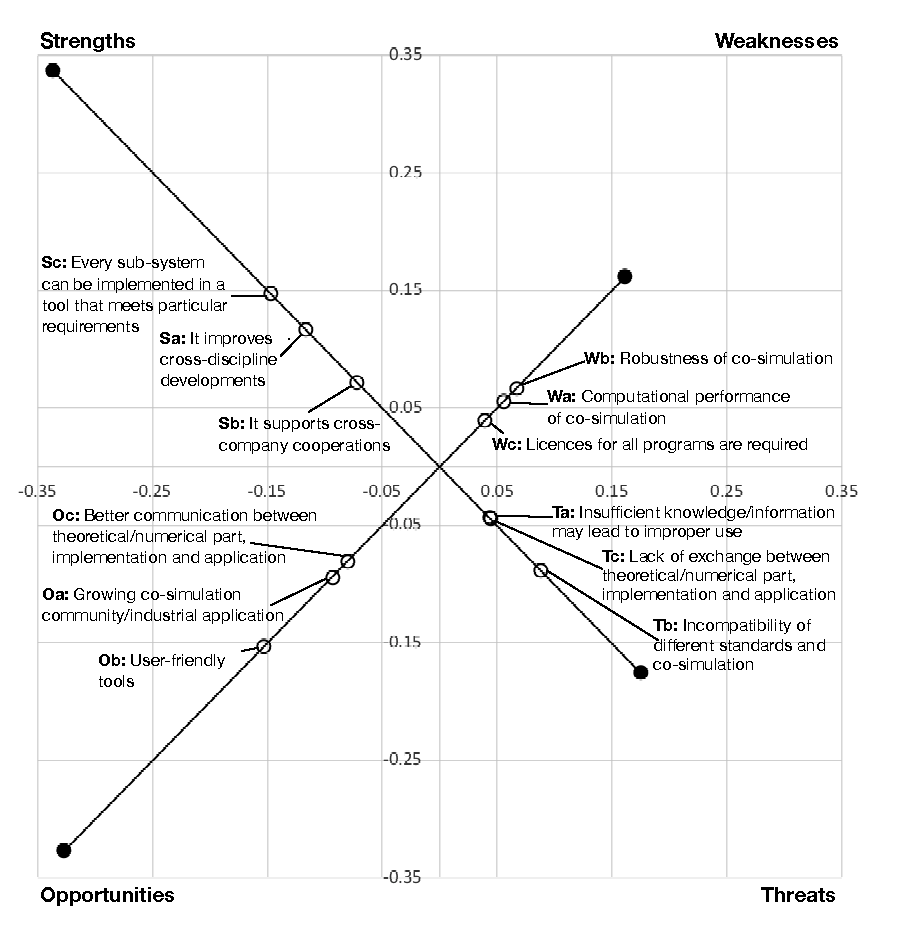
\includegraphics[width=1\textwidth]{Figures/SWOTAHPcosim.eps}
\caption{Research needs}
\label{fig:SWOT}
\end{figure}


The results of the SWOT-AHP analysis indicate that strengths and opportunities factors predominate. The four factors with the highest global priorities are within the Strengths and Opportunities group. The factor with the highest global priority is the external opportunity of User-friendly tools including pre-defined master algorithms, integrated error estimation, etc. The factor with the second highest global priority is the internal strengths that sub-systems can be implemented in a tool that meets the particular requirements for the domain, the structure of the model and the simulation algorithm. The factor with the third highest global priority is the internal strengths that co-simulation supports cross-discipline developments. Some experts mentioned further SWOT factors. As a strengths, some experts mentioned that parallel modeling and simulation can reduce the overall modeling and simulation time. Another strength is that co-simulation approaches supports modularity and the reuse of components. An expert stated the lack of sufficiently strong theory as a weakness of co-simulation. In the group opportunities, an expert mentioned the integration of tools for the application of formal methods. On expert pointed out that a threat could be that some big companies may be actively against the widespread use of co-simulation.

An interesting outcome is that the groups of Strengths and Opportunities are seen much more important than Weaknesses and threats. This follows due to the priority of the first two groups, which are approximately twice as high as the latter two. The consistencies of the pairwise comparisons was checked. All consistency ratios are below xxx. It can be concluded, that the results are consistent. 

\claudio{It's strange that so many people use FMI for discrete event co-simulation... and at the same time the FMI committee is trying to improve the standard to support DE based co-simulation! 
As a result, a critic we might get in our study is that there is no balance in the selection of experts.
We must defend from this criticism in the discussion section.}



%\claudioi{Also, overall we should summarize the results as we introduce each figure/table. So that the reader can opt for just read the text (ignore the figs) and still get a sense of what the main results are.}

%\claudioi{To follow good practice, every figure/table must be within a float environment. If we need to keep figures within a specific section, then we should use the appropriate positioning parameters (and the float package).}

